\documentclass[11pt]{article}

\usepackage[a4paper,margin=0.85in]{geometry}
\usepackage{amsmath}
\usepackage{booktabs}
\usepackage{caption}
\usepackage{float}
\usepackage{gensymb}
\usepackage{graphicx}
\usepackage[numbers]{natbib}
\usepackage{tabularx}
\usepackage{url}

\emergencystretch=3em
\setlength{\parindent}{0pt}
\setlength{\parskip}{0.55em}
\captionsetup{font=small,labelfont=bf}
\renewcommand{\thesection}{S\arabic{section}}
\renewcommand{\thetable}{S\arabic{table}}
\renewcommand{\thefigure}{S\arabic{figure}}

\begin{document}

\begin{center}
{\Large\bfseries Supplementary Material}\\[0.45em]
{\large Hidden Behind the Mean: Probabilistic Diagnostics of Discomfort-Relevant Thermal-Sensation Tails Under Future Weather}\\[0.45em]
Hongshan Guo et al.
\end{center}

\vspace{0.5em}
\hrule
\vspace{0.8em}

\section{Scope}

This supplementary material documents validation and reproducibility checks for the diagnostic analyses in the main manuscript. It does not report closed-loop control, energy savings, demand-response performance, or equipment-facing outcomes.

\section{Run Inventory and Trace Integrity}

The final diagnostic run contains 144 annual DOE Medium Office selection-role cases: six cities, two emissions scenarios, four time slices, and three annual weather-file severities. These role-labelled cases represent 119 unique source-year weather trajectories. Each annual trace contains 35{,}040 15-minute rows and 16{,}704 occupied rows. The zone-raw trace schema contains 45 raw environmental fields: air temperature, mean radiant temperature, and relative humidity for each of 15 conditioned zones.

The source IDF was \texttt{ASHRAE901\_OfficeMedium\_STD2019\_Denver.idf}. Each annual run used four timesteps per hour. The run period was assigned a Monday start, with weather-file holidays and daylight-saving adjustments disabled, so the common weekday 06:00--22:00 screen yields 16{,}704 occupied rows per case. The API applied 22/24\,\degree C occupied heating/cooling setpoints and 12/30\,\degree C unoccupied setpoints. EnergyPlus used each EPW's location metadata, but zone, system, and plant sizing retained the source IDF's Denver heating and cooling design days. The analysis is therefore a fixed-design-basis stress test rather than a set of locally resized prototypes.

The final zone-raw diagnostic run produced 144 per-case trace files, 144 EnergyPlus error files, and 144 EnergyPlus end files. All annual cases completed without fatal EnergyPlus errors. Sixteen cases reported warmup load-convergence Severe messages; these cases completed successfully and are retained with this quality-assurance note.

\subsection*{Same-state temporal alignment audit}

The original online trace placed diagnostic outputs generated at the beginning-of-zone-timestep callback and environmental fields recorded at the end-of-zone-timestep callback on the same CSV row. Revision-stage reproducibility QA identified this callback-order mismatch. All manuscript-facing PMV, primary ordinal, no-PMV ordinal, nominal, and endpoint probability quantities were therefore regenerated from the common recorded end-of-zone-timestep state. The EnergyPlus simulations, weather inputs, and environmental state histories were not rerun or changed, and the original online diagnostic columns remain preserved for audit rather than reused.

The synchronized analysis completed 144/144 role cases and mapped them to 119 unique checksum-identified state arrays, each with 16{,}704 occupied rows and 15 conditioned zones. All required arrays were finite and schema-valid, and duplicate selection roles produced identical results. At the manuscript screen, synchronization changed mean-zone, any-zone, and mean-hidden any-zone shares from 13.448\%, 37.032\%, and 23.584\% in the original callback-timed columns to 13.147\%, 36.643\%, and 23.496\%, respectively. The correction altered no prespecified spatial ordering or future-slice direction.

\section{Weather Panel and Case Provenance}

The weather panel is used as a deterministic stress-test panel, not as a probabilistic climate ensemble. The 144 cases are the Cartesian product of six cities (Ahmedabad, Beijing, Guangzhou, Houston, Kolkata, and Phoenix), two emissions scenarios (SSP2-4.5 and SSP5-8.5), four candidate windows (reference 2025--2029, near 2030--2039, mid 2050--2059, and late 2080--2089), and three selected annual severities (typical, hot, and heatwave-extreme). The three annual severities are independently applied selection labels within the local weather-file generation workflow; they should not be read as equal-probability climate outcomes. The five-year reference window is retained as the file label \texttt{baseline\_2020s}, while each later window contains ten candidate years. In 24 of the 48 city--scenario--time-slice groups, the hot and heatwave-extreme roles select the same source year; in one additional group, the typical and heatwave-extreme roles coincide. The 144 selection-role files therefore represent 119 unique source-year trajectories.

Primary results retain the prespecified selection-role weighting. As a complementary check, each unique source-year trajectory was counted once (equivalently, overlapping roles received inverse-multiplicity weights). Table~\ref{tab:supp_unique_weather} shows that this reduced absolute screening rates modestly without changing the spatial-aggregation result.

\begin{table}[htbp]
\centering
\caption{Selection-role and unique-source-year weighting sensitivity.}
\label{tab:supp_unique_weather}
\footnotesize
\begin{tabular}{lrrr}
\toprule
Metric & 144 role labels & 119 unique years & Difference \\
\midrule
Mean $p_{\mathrm{tail}}$ & 0.1156 & 0.1132 & -0.0024 \\
Mean-zone high-tail (\%) & 13.15 & 12.44 & -0.71 \\
Any-zone high-tail (\%) & 36.64 & 35.41 & -1.23 \\
Hidden any-zone high-tail (\%) & 23.50 & 22.98 & -0.52 \\
Area-weighted zone-time high-tail (\%) & 12.87 & 12.18 & -0.69 \\
\bottomrule
\end{tabular}
\end{table}

The preserved archive contains 12 hourly forecast series spanning 2025--2100, one per city--scenario pair, and paired workbooks. All 12 workbooks identify MPI-ESM1-2-LR, \texttt{rcm=N/A}, a 1991--2010 baseline, and documented daily climate-delta transformations for dry-bulb temperature, pressure, wind speed, and GHI. For each candidate window, the executable selector chooses the year nearest median annual CDH18 for the typical role, maximum annual CDH18 for the hot role, and maximum hours with dry-bulb temperature at or above 35\,\degree C for the heatwave-extreme role. Ties in the latter are resolved by annual maximum temperature and then CDH18. The legacy source-field label \texttt{CDD18\_hourly} stores CDH18 in degree-Celsius hours, not conventional degree-days; dividing it by 24 changes units but not the selection ranking.

The EPW converter copies dry-bulb temperature, relative humidity, pressure, global horizontal radiation, direct normal radiation, diffuse horizontal radiation, and wind speed from the forecast output; converts pressure from hPa to Pa; computes dew point from dry bulb and relative humidity; and assigns explicit sentinel or default values to unsupported EPW fields. Revision-stage QA reproduced 144/144 manifest selections and the exact source-to-EPW transformation for 119/119 unique selected source years. All 12 source series passed structural and broad plausibility checks with no logged issue. All 144 EPWs passed row-count, field-width, broad physical-range, and dew-point-consistency checks. Artifact checksums, selector outputs, transformation checks, and the weather-role overlap table are retained with the revision analysis.

An exact paired comparison of each city's two scenario files found that relative humidity, specific humidity, and direct-normal irradiance were identical at all 666{,}169 matched timestamps; dry-bulb temperature, pressure, wind speed, GHI, and diffuse horizontal radiation differed. The converter does not write the source specific-humidity field. It carries relative humidity into the EPW and calculates dew point from the future dry-bulb temperature and that carried relative humidity, so absolute moisture changes mechanically under an effectively fixed-RH assumption. Direct-normal irradiance is also carried without a scenario-specific signal. Consequently, the panel supports joint-weather-file stress testing but not attribution to independently projected humidity or direct-beam changes. Horizontal GHI is retained only as a descriptive forcing variable and is not interpreted as facade-incident solar gain.

The broader archive contains a matching climate-delta generator implementation whose mixed-resolution daily-delta method, metadata, output schema, and MPI-ESM1-2-LR loading path align with the 12 preserved workbooks. The method family has also been evaluated against 2011--2020 observations across benchmark cities and forcing sources, with a companion decomposition of baseline-source, climate-signal-resolution, and downstream degree-day effects \citep{GuoHe2026sAMY,GuoHe2026InputQuality}. The exact six-city study-batch configuration and its raw CMIP6 and observational inputs are not preserved with these outputs. The audit therefore supports algorithmic lineage and exact regeneration from the frozen hourly forecast artifacts through selection and EPW conversion, but not byte-level end-to-end regeneration or exact-file external validation. The panel also uses one GCM forcing family and is not a climate-model uncertainty ensemble. Structural and range checks establish integrity and broad plausibility, not predictive validity.

The reproducibility package will archive the run manifest, weather-file provenance table, case identifiers, trace-schema checks, and checksum records needed to audit the mapping between manuscript cases and generated annual weather files. Large weather files and per-timestep traces may be represented by checksums rather than redistributed directly where file size or third-party restrictions apply.

\section{Panel-Level Conditional Uncertainty}

Uncertainty summaries use independent design units rather than treating 15-minute timesteps as independent. For panel-wide and spatial summaries, 10{,}000 fixed-seed bootstrap draws resampled 48 city--scenario--time-slice blocks while retaining all three weather-selection roles within each sampled block. Time-slice contrasts resampled 12 city--scenario blocks with all four slices retained. A separate sensitivity gave each of the 119 distinct environmental states equal weight while retaining those states within their parent design blocks. The resulting 2.5th--97.5th percentile ranges quantify conditional case composition; they do not include climate-model, weather-construction, model-refitting, building, or future-occupant structural uncertainty.

\begin{table}[htbp]
\centering
\caption{Corrected same-state panel summaries with conditional block-bootstrap percentile ranges.}
\label{tab:supp_panel_uncertainty}
\footnotesize
\begin{tabular}{lrr}
\toprule
Metric & 144 role labels & 119 unique states \\
\midrule
Mean-zone high-tail (\%) & 13.15 [11.02, 15.45] & 12.44 [10.60, 14.47] \\
Any-zone high-tail (\%) & 36.64 [32.39, 40.87] & 35.41 [31.66, 39.31] \\
Hidden any-zone high-tail (\%) & 23.50 [20.79, 26.12] & 22.98 [20.55, 25.52] \\
\bottomrule
\end{tabular}
\end{table}

\begin{table}[htbp]
\centering
\caption{Paired differences in mean-zone high-tail share. Ranges are conditional block-bootstrap percentiles in percentage points.}
\label{tab:supp_panel_contrasts}
\footnotesize
\begin{tabular}{lr}
\toprule
Contrast & Difference [2.5th, 97.5th percentile] \\
\midrule
Near-2030s minus reference & $-0.02$ [$-2.00$, 1.70] \\
Mid-2050s minus reference & $+5.05$ [1.81, 9.03] \\
Late-2080s minus reference & $+11.93$ [8.10, 16.31] \\
SSP5-8.5 minus SSP2-4.5 & $+3.40$ [2.28, 4.37] \\
\bottomrule
\end{tabular}
\end{table}

The scenario contrast has only six paired city resampling units and is explicitly conditional on the tested cities. It is not an interval for regional or global SSP uncertainty. The near-2030s contrast includes zero, whereas the mid- and late-century contrasts remain positive under this finite-panel resampling.

\section{TSV Corpus and Study-Specific Predictor}

The study-specific predictor was fitted to 148{,}148 pooled field observations: 106{,}171 from the ASHRAE Global Thermal Comfort Database II and 41{,}977 from the Chinese Thermal Comfort Dataset. Thermal-sensation values were rounded to the nearest integer class and clipped to the seven-point range. All 148{,}148 rows in the harmonized analysis corpus entered the TSV-stratified random split (seed 42) shown in Table~\ref{tab:supp_corpus_split}.

\begin{table}[htbp]
\centering
\caption{Source composition of the study-specific model partitions.}
\label{tab:supp_corpus_split}
\footnotesize
\begin{tabular}{lrrr}
\toprule
Partition & ASHRAE & China & Total \\
\midrule
Training (70\%) & 74{,}320 & 29{,}383 & 103{,}703 \\
Calibration (15\%) & 15{,}885 & 6{,}337 & 22{,}222 \\
Held-out test (15\%) & 15{,}966 & 6{,}257 & 22{,}223 \\
\midrule
Total & 106{,}171 & 41{,}977 & 148{,}148 \\
\bottomrule
\end{tabular}
\end{table}

For field-corpus model development, all preprocessing quantities were estimated from the training partition. Missing or non-numeric predictors were replaced by training medians. Body-surface-area values outside 1--3\,m$^2$ were replaced by Du~Bois estimates using bounded height and weight values; otherwise the training median was retained. Prespecified physical ranges were then enforced, and air temperature, mean radiant temperature, air speed, relative humidity, metabolic rate, clothing insulation, body surface area, and prevailing outdoor mean temperature were winsorized at their training-set 1st and 99th percentiles. The derived feature vector was standardized using training-partition means and standard deviations. The serialized model artifact retains the fitted medians, winsorization bounds, feature scaler, learners, and calibrators.

For the 15-minute simulation application, the running mean was initialized from the first post-warmup outdoor-air temperature and updated as \(T_{\mathrm{rm},t}=\alpha T_{\mathrm{rm},t-1}+(1-\alpha)T_{\mathrm{out},t}\), where \(\alpha=0.8^{1/96}\). Let $T_{\mathrm{op}}=(T_a+T_r)/2$ and $T_n=0.31T_{\mathrm{rm}}+17.8$. Define $\Delta w=0$ unless $T_{\mathrm{op}}>25\,\degree C$ and $v\ge0.3$\,m/s; under that condition, $\Delta w=1.2$, 1.8, or 2.2 for $0.3\le v<0.9$, $0.9\le v<1.2$, or $v\ge1.2$\,m/s, respectively. With $w=3.5+\Delta w$ when $T_{\mathrm{op}}\ge T_n$ and $w=3.5$ otherwise, define $s=(T_{\mathrm{op}}-T_n)/w$. The fitted feature vector is
\begin{equation}
\mathbf{x}=\left(T_{\mathrm{op}},v,\mathrm{RH},\mathrm{met}_c,\mathrm{clo}_c,
\mathrm{met}_c\mathrm{clo}_c,\mathrm{BSA},\Delta w,
\operatorname{clip}(s,-1,1),\max(-s-1,0),\mathrm{PMV},s\right),
\end{equation}
where $\mathrm{met}_c$ and $\mathrm{clo}_c$ are centered using their training-partition means. These outdoor-context terms are predictor covariates, not an adaptive-comfort compliance test. The no-PMV sensitivity model removes only PMV from this vector.

Each simulated occupied-zone state supplied EnergyPlus air temperature, mean radiant temperature, and relative humidity together with fixed inputs \(v=0.10\) m/s, \(\mathrm{met}=1.10\), \(\mathrm{clo}=0.65\), and \(\mathrm{BSA}=1.80\) m$^2$. The application path applied the stated physical-range constraints and the fitted feature standardization; the percentile winsorization above describes field-corpus preprocessing.

The ordinal predictor comprises six LightGBM binary heads estimating $\Pr(Y>k)$ for $k=-3,\ldots,+2$. Each head was fitted on the training partition and calibrated independently by prefit isotonic regression on the calibration partition. The calibrated cumulative probabilities were constrained to be non-increasing across thresholds, differenced to recover the seven class probabilities, and normalized. Table~\ref{tab:supp_model_settings} reports the fixed study-specific settings.

\begin{table}[htbp]
\centering
\caption{Effective settings of the study-specific ordinal predictor.}
\label{tab:supp_model_settings}
\footnotesize
\begin{tabularx}{\textwidth}{@{}p{0.35\textwidth}X@{}}
\toprule
Setting & Value \\
\midrule
Learner & Six binary LightGBM cumulative heads \\
Trees per head; learning rate & 400; 0.05 \\
Maximum depth; leaves & Unlimited ($-1$); 31 \\
Minimum child samples & 20 \\
Column sampling & 0.90 \\
Row bagging & None in the effective fit (\texttt{subsample\_freq}=0) \\
L1; L2 regularization & 0; 0 \\
Class weighting/resampling & None \\
Calibration & Separate prefit isotonic regression per cumulative head \\
Random seed; early stopping & 42; none \\
Hyperparameter search & None for the study-specific fit \\
Software & Python 3.11.5; LightGBM 4.5.0; scikit-learn 1.4.2; NumPy 1.26.4; pandas 2.2.3; pythermalcomfort 2.10.0 \\
PMV implementation & pythermalcomfort \texttt{pmv\_ppd}; ISO/SI; \texttt{limit\_inputs=False} \\
\bottomrule
\end{tabularx}
\end{table}

\section{Metabolic Profiles}

The metabolic-spread diagnostic reuses the same simulated environmental traces and re-evaluates the TSV probability model under six metabolic-load profiles: 90.0, 93.2, 100.0, 108.0, 110.0, and 120.0 W/person. Using 1\,met${}=58.2$\,W/m$^2$ and a fixed body surface area of \(120/(1.2\times58.2)=1.718\) m$^2$, the six profiles correspond to 0.900, 0.932, 1.000, 1.080, 1.100, and 1.200 met. Body surface area remains fixed across this profile comparison. These profiles are sensitivity cases for the reported-TSV model. EnergyPlus was not rerun with altered internal heat gains, and the profiles are not demographic strata assigned to simulated occupants.

\section{Held-Out TSV Prediction Validation}

The primary TSV predictor and the no-PMV robustness predictor were evaluated on the same held-out pooled-corpus test partition of 22{,}223 records (15{,}966 ASHRAE and 6{,}257 China). This TSV-stratified record-level split is internal validation rather than source-held-out external validation. The rounded-PMV baseline rounds PMV to the nearest TSV class and clips the value to $[-3,+3]$; it is a deterministic scalar-label baseline, not a calibrated probability model.

\begin{table}[htbp]
\centering
\caption{Held-out TSV validation for the primary predictor, no-PMV robustness predictor, and rounded-PMV class baseline. Argmax-tail metrics first assign the most probable TSV class and then group classes by tail status; they are distinct from the probability-screen F1 in Table~\ref{tab:supp_tail_probability_comparison}.}
\label{tab:supp_tsv_validation}
\scriptsize
\setlength{\tabcolsep}{3.2pt}
\begin{tabular}{lrrrrrrr}
\toprule
Predictor & Exact (\%) & Within $\pm1$ (\%) & MAE & Argmax-tail recall (\%) & Argmax-tail F1 (\%) & Log loss & Tail MAE \\
\midrule
Primary TSV model & 47.3 & 84.1 & 0.73 & 23.4 & 34.0 & 1.454 & 0.277 \\
No-PMV TSV model & 46.9 & 83.8 & 0.73 & 23.1 & 33.5 & 1.476 & 0.278 \\
Rounded PMV class & 33.2 & 76.5 & 0.97 & 22.8 & 26.6 & -- & 0.258 \\
\bottomrule
\end{tabular}
\end{table}

\begin{table}[H]
\centering
\caption{Observed class support and class-specific recall on the held-out test partition. Values are percentages except support counts.}
\label{tab:supp_class_recall}
\scriptsize
\setlength{\tabcolsep}{4.2pt}
\begin{tabular}{lrrrrrrr}
\toprule
Predictor & TSV -3 & TSV -2 & TSV -1 & TSV 0 & TSV +1 & TSV +2 & TSV +3 \\
\midrule
Support ($n$) & 443 & 1238 & 3755 & 9834 & 4064 & 1982 & 907 \\
Primary TSV model & 25.5 & 6.9 & 12.4 & 88.0 & 16.2 & 15.7 & 23.9 \\
No-PMV TSV model & 23.7 & 6.5 & 13.0 & 87.4 & 15.4 & 15.8 & 23.2 \\
Rounded PMV class & 13.8 & 10.4 & 27.6 & 47.8 & 26.3 & 14.5 & 10.5 \\
\bottomrule
\end{tabular}
\end{table}

\section{Calibrated Tail-Probability Comparison}

As a scalar-reference check, PMV was also given a calibrated probability baseline. This baseline used only $|\mathrm{PMV}|$ as the input and the binary tail label $\mathbf{1}\{\mathrm{TSV}\le-2\ \mathrm{or}\ \mathrm{TSV}\ge+2\}$ as the target. An isotonic regression was fitted on the non-test partition and evaluated on the same held-out test records used in Tables~\ref{tab:supp_tsv_validation} and~\ref{tab:supp_class_recall}. This is not an ordinal TSV model; it only tests how much TSV-tail probability can be recovered from PMV alone after calibration. Table~\ref{tab:supp_tail_probability_comparison} compares that scalar baseline with the primary and no-PMV TSV probability models using the same tail-probability metrics.

\begin{table}[htbp]
\centering
\caption{Held-out tail-probability comparison for the TSV probability models and the PMV-only calibrated scalar baseline. F1 is computed by screening each predicted tail probability at $p_{\mathrm{tail}}\ge0.20$.}
\label{tab:supp_tail_probability_comparison}
\scriptsize
\setlength{\tabcolsep}{3.2pt}
\begin{tabular}{lrrrrrrrrr}
\toprule
Predictor & $n$ & Mean predicted & Observed & Brier & ECE & MCE & F1 (\%) & AUROC & Avg. precision \\
\midrule
Primary TSV model & 22223 & 0.207 & 0.206 & 0.137 & 0.011 & 0.047 & 47.1 & 0.747 & 0.487 \\
No-PMV TSV model & 22223 & 0.207 & 0.206 & 0.138 & 0.006 & 0.012 & 46.4 & 0.747 & 0.483 \\
PMV-only calibrated tail baseline & 22223 & 0.206 & 0.206 & 0.161 & 0.003 & 0.017 & 32.6 & 0.571 & 0.260 \\
\bottomrule
\end{tabular}
\end{table}

The PMV-only baseline matched the overall tail prevalence after calibration, with mean predicted $p_{\mathrm{tail}}=0.206$ and observed tail frequency $0.206$. Its calibration error was low, but its discrimination was limited: AUROC was 0.571 and average precision was 0.260, compared with AUROC 0.747 and average precision 0.483--0.487 for the TSV probability models. This supports the limited interpretation in the main text: PMV contains useful scalar information, but PMV alone is not the same diagnostic object as a calibrated TSV probability distribution.

\section{Contributor-Clustered Held-Out Uncertainty}

The pooled test split contains 63 contributor groups. To avoid treating repeated records from one contributor as independent for interval calculation, 5{,}000 fixed-seed bootstrap draws sampled contributors with replacement and assigned a common multiplicity to all of their held-out records. These conditional percentile intervals quantify held-out contributor composition; they do not propagate model-refitting uncertainty or establish contributor-level transport because the original model split was record-level.

Table~\ref{tab:supp_heldout_cluster_contrasts} reports paired model contrasts for both the primary outer-category event and the endpoint-only event. The endpoint event contains 1{,}350 observed records (443 at TSV $-3$ and 907 at TSV $+3$) among 22{,}223 test records. Its support is therefore lower than that of the primary event but sufficient for a bounding sensitivity.

\begin{table}[htbp]
\centering
\caption{Contributor-clustered paired held-out contrasts. Values are point difference [2.5th, 97.5th conditional bootstrap percentiles]. Brier differences below zero and discrimination differences above zero favor the primary predictor.}
\label{tab:supp_heldout_cluster_contrasts}
\scriptsize
\setlength{\tabcolsep}{2.0pt}
\begin{tabular}{llrrr}
\toprule
Event & Comparator & Brier & AUROC & Avg. precision \\
\midrule
$|\mathrm{TSV}|\ge2$ & PMV-only & $-0.0235$ [$-0.0293,-0.0180$] & $+0.1767$ [$+0.1375,+0.2034$] & $+0.2271$ [$+0.1863,+0.2597$] \\
$|\mathrm{TSV}|\ge2$ & No-PMV TSV & $-0.0003$ [$-0.0010,+0.0002$] & $+0.0008$ [$-0.0023,+0.0035$] & $+0.0044$ [$-0.0009,+0.0102$] \\
TSV $\in\{-3,+3\}$ & PMV-only & $-0.0094$ [$-0.0148,-0.0050$] & $+0.1810$ [$+0.1314,+0.2212$] & $+0.2602$ [$+0.1706,+0.3276$] \\
TSV $\in\{-3,+3\}$ & No-PMV TSV & $+0.0000$ [$-0.0003,+0.0004$] & $-0.0030$ [$-0.0077,+0.0013$] & $+0.0005$ [$-0.0084,+0.0091$] \\
\bottomrule
\end{tabular}
\end{table}

For the primary endpoint probability, Brier score was 0.0465 [0.034, 0.057], AUROC was 0.819 [0.773, 0.858], and average precision was 0.370 [0.250, 0.481]. The endpoint result is therefore retained as a support-limited definition sensitivity, not as a replacement outcome or a validated dissatisfaction probability. For both event definitions, the primary-versus-no-PMV intervals include zero, so the two TSV predictors are described as closely performing variants rather than ranked models.

\section{Predictor-Form and Tail-Definition Sensitivity}

The saved nominal seven-class predictor was applied to exactly the same synchronized state arrays as the primary ordinal predictor. Table~\ref{tab:supp_model_form_panel} shows that the central spatial ordering is preserved at the manuscript screen. Its area-weighted mean-probability column applies the threshold after spatial probability averaging and is distinct from the area-weighted zone-time screened share reported in Table~\ref{tab:supp_unique_weather}. Absolute agreement is threshold-dependent: at $\tau=0.10$, the nominal-minus-ordinal difference reaches 11.05 percentage points for the any-zone statistic, whereas the largest difference at $\tau=0.20$ is 1.48 points. The robustness result is therefore directional rather than numerical equivalence across model forms.

\begin{table}[htbp]
\centering
\caption{Panel screening rates by probability-model specification at $\tau=0.20$.}
\label{tab:supp_model_form_panel}
\footnotesize
\begin{tabular}{lrrrrr}
\toprule
Predictor & Mean-zone & Area-weighted mean-prob. & p90-zone & Any-zone & Hidden any-zone \\
\midrule
Primary ordinal & 13.15 & 12.13 & 27.83 & 36.64 & 23.50 \\
Nominal seven-class & 14.34 & 12.74 & 27.86 & 35.16 & 20.82 \\
No-PMV ordinal & 13.85 & 12.76 & 29.09 & 37.52 & 23.67 \\
\bottomrule
\end{tabular}
\end{table}

The stricter endpoint event uses only \(p_{\mathrm{outermost}}=p_{-3}+p_{+3}\). Table~\ref{tab:supp_endpoint_panel} shows that its absolute rates are highly sensitive to the probability screen, but the any-zone-minus-mean-zone gap remains positive at every prespecified screen. This rules out the interpretation that the spatial result is created solely by including TSV $\pm2$, while the sparse endpoint labels preclude treating the endpoint event as a better-supported replacement.

\begin{table}[htbp]
\centering
\caption{Endpoint-only spatial sensitivity with conditional block-bootstrap ranges for the mean-hidden any-zone gap.}
\label{tab:supp_endpoint_panel}
\footnotesize
\begin{tabular}{rrrr}
\toprule
Endpoint screen & Mean-zone (\%) & Any-zone (\%) & Hidden gap [2.5th, 97.5th] (pp) \\
\midrule
0.025 & 33.30 & 69.33 & 36.03 [34.58, 37.48] \\
0.050 & 10.99 & 30.34 & 19.35 [17.26, 21.37] \\
0.075 & 3.79 & 23.87 & 20.08 [17.51, 22.58] \\
0.100 & 1.42 & 20.30 & 18.88 [16.14, 21.56] \\
0.150 & 0.12 & 7.65 & 7.53 [5.84, 9.28] \\
0.200 & 0.04 & 0.74 & 0.70 [0.41, 1.04] \\
\bottomrule
\end{tabular}
\end{table}

\section{Contributor-Grouped Robustness Check}

The record-level split above tests held-out records under the same overall pooled ASHRAE--China data distribution. As a stricter robustness check, the ordinal predictors were also re-estimated under five contributor-grouped train/calibration/test splits. Contributor groups were kept disjoint across training, calibration, and test partitions. Each split used 43 contributor groups for training, 10 for calibration, and 10 for testing; the mean test size was 26{,}484 records.

This grouped check uses the same 400-tree specification as the application model and is not used as the main model-selection criterion because contributor groups differ substantially in geography, building type, measurement protocol, and class balance. It is included to expose domain-transfer sensitivity. Performance was lower than under the record-level split, especially for tail-event discrimination, but the primary and no-PMV feature sets remained similar. Tail F1 uses the same diagnostic screen as the application analysis, \(p_{\mathrm{tail}}\ge0.20\), rather than classifying the probability-vector argmax as central or tail.

\begin{table}[htbp]
\centering
\caption{Contributor-grouped validation over five disjoint-group splits using the study-specific 400-tree specification. Values are mean (standard deviation) across splits. F1 uses \(p_{\mathrm{tail}}\ge0.20\).}
\label{tab:supp_grouped_validation}
\scriptsize
\setlength{\tabcolsep}{2.7pt}
\begin{tabular}{lrrrrrrrr}
\toprule
Feature set & Exact (\%) & Within $\pm1$ (\%) & MAE & Brier & ECE & AUROC & Avg. precision & F1 (\%) \\
\midrule
Primary & 42.1 (2.8) & 79.8 (2.1) & 0.832 (0.044) & 0.174 (0.012) & 0.061 (0.025) & 0.577 (0.021) & 0.290 (0.035) & 32.5 (4.3) \\
No-PMV & 41.9 (2.9) & 79.4 (1.7) & 0.839 (0.038) & 0.174 (0.012) & 0.058 (0.022) & 0.580 (0.020) & 0.285 (0.026) & 34.2 (4.5) \\
\bottomrule
\end{tabular}
\end{table}

\section{Overlap-Excluded Reciprocal Source-Label Holdout Check}

To examine transport across the two source labels without target-corpus fitting, the study-specific pipeline was re-estimated in both directions. Six normalized city--year strata with evidence of likely cross-source study overlap were first excluded from both corpora, leaving 104{,}354 ASHRAE and 40{,}421 China-labelled records. The named source corpus was then divided into 82.35\% training and 17.65\% calibration subsets, preserving the pooled fit's 70:15 train-to-calibration ratio. All preprocessing statistics, LightGBM fitting, and isotonic calibration were estimated from the source corpus alone. The target corpus was reserved in full for evaluation, with no target-corpus recalibration or fine-tuning.

\begin{table}[H]
\centering
\caption{Overlap-excluded reciprocal source-label holdout results for the primary ordinal predictor. Observed/predicted reports target-corpus tail prevalence and mean predicted $p_{\mathrm{tail}}$; F1 uses the $p_{\mathrm{tail}}\ge0.20$ screen.}
\label{tab:supp_source_holdout}
\scriptsize
\setlength{\tabcolsep}{2.5pt}
\begin{tabular}{lrrrrrrrr}
\toprule
Direction & $n$ & Exact (\%) & Within $\pm1$ (\%) & MAE & Observed/predicted & ECE & AUROC & F1 (\%) \\
\midrule
ASHRAE$\rightarrow$China & 40{,}421 & 42.9 & 81.9 & 0.800 & 0.165/0.225 & 0.096 & 0.592 & 31.3 \\
China$\rightarrow$ASHRAE & 104{,}354 & 39.8 & 77.8 & 0.886 & 0.223/0.121 & 0.124 & 0.553 & 25.2 \\
\bottomrule
\end{tabular}
\end{table}

Tail-event discrimination and calibration were weaker than under the pooled record-level split, and the direction of the observed/predicted gap differed across the two target corpora. Class-distance metrics did not consistently improve on an always-neutral target baseline. A calibrated nominal seven-class comparator was as good or better on most source-shift metrics (tail AUROC 0.596 and 0.560; ECE 0.077 and 0.116), so no ordinal-algorithm superiority is inferred. Metadata matching cannot exclude all shared studies, and the retained ASHRAE-labelled subset includes 4{,}426 observations collected in China. The result is therefore evidence of material source-label sensitivity, not geography-independent or third-corpus external validation.

\section{TSV-Tail Probability Calibration}

The central probability variable in the manuscript is
\begin{equation}
p_{\mathrm{tail}}=\Pr(\mathrm{TSV}\le-2)+\Pr(\mathrm{TSV}\ge+2).
\end{equation}
To check whether this value behaves as a calibrated probability on held-out data, predicted $p_{\mathrm{tail}}$ values were grouped into fixed probability bins. Within each bin, the mean predicted $p_{\mathrm{tail}}$ was compared with the observed frequency of tail-class records. Tail expected calibration error (ECE) is the bin-count-weighted mean absolute difference between predicted and observed frequency. Tail maximum calibration error (MCE) is the largest bin-level absolute difference.

\begin{table}[htbp]
\centering
\caption{Held-out calibration summary for predicted TSV-tail probability.}
\label{tab:supp_tail_calibration_summary}
\footnotesize
\setlength{\tabcolsep}{4.5pt}
\begin{tabular}{lrrrrrr}
\toprule
Predictor & $n$ & Mean predicted & Observed & Tail Brier & Tail ECE & Tail MCE \\
\midrule
Primary TSV model & 22223 & 0.207 & 0.206 & 0.137 & 0.011 & 0.047 \\
No-PMV TSV model & 22223 & 0.207 & 0.206 & 0.138 & 0.006 & 0.012 \\
\bottomrule
\end{tabular}
\end{table}

\begin{figure}[htbp]
\centering
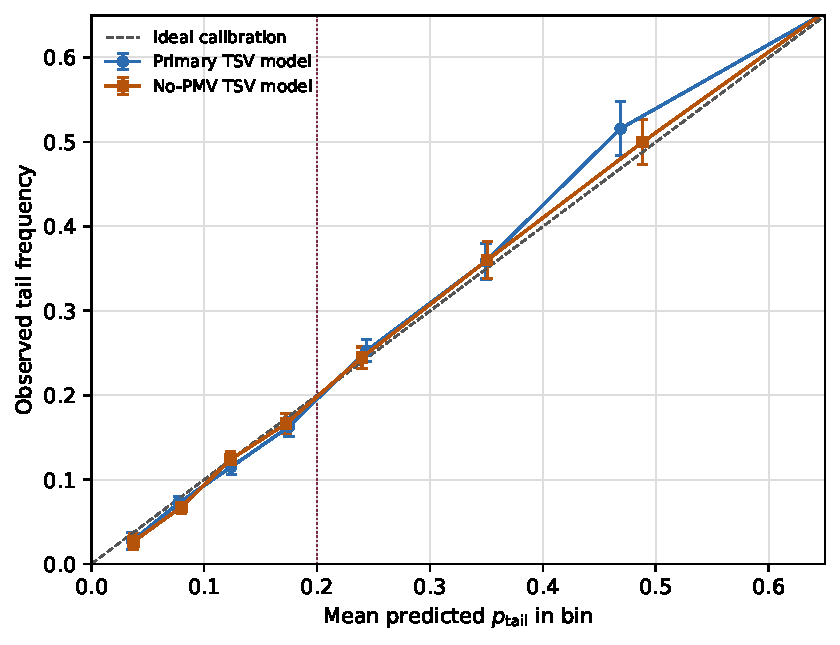
\includegraphics[width=0.68\textwidth]{figs/p_tail_calibration_reliability.pdf}
\caption{Held-out reliability check for predicted TSV-tail probability. Points show fixed bins of predicted $p_{\mathrm{tail}}$; vertical bars show approximate 95\% binomial intervals for the observed tail frequency in each bin. The dashed line marks ideal calibration, and the dotted vertical line marks the manuscript's illustrative reporting screen $p_{\mathrm{tail}}=0.20$.}
\label{fig:supp_tail_calibration}
\end{figure}

\begin{table}[htbp]
\centering
\caption{Primary TSV model: fixed-bin held-out calibration for $p_{\mathrm{tail}}$.}
\label{tab:supp_primary_tail_bins}
\footnotesize
\begin{tabular}{lrrrr}
\toprule
Bin & $n$ & Mean predicted & Observed & Abs. error \\
\midrule
0.00--0.05 & 1024 & 0.036 & 0.027 & 0.009 \\
0.05--0.10 & 4021 & 0.077 & 0.072 & 0.005 \\
0.10--0.15 & 4652 & 0.124 & 0.115 & 0.009 \\
0.15--0.20 & 4251 & 0.175 & 0.163 & 0.012 \\
0.20--0.30 & 4277 & 0.244 & 0.253 & 0.009 \\
0.30--0.40 & 2005 & 0.350 & 0.359 & 0.009 \\
0.40--0.60 & 919 & 0.469 & 0.516 & 0.047 \\
0.60--1.00 & 1074 & 0.713 & 0.701 & 0.012 \\
\bottomrule
\end{tabular}
\end{table}

The held-out calibration check supports using $p_{\mathrm{tail}}$ as a diagnostic probability rather than only as an uncalibrated score. The primary model's mean predicted $p_{\mathrm{tail}}$ was 0.207, close to the observed held-out tail frequency of 0.206. Fixed-bin ECE was 0.011 for the primary predictor and 0.006 for the no-PMV predictor. These values do not remove the sparse-tail limitation noted in the manuscript, but they show that the aggregate tail probability is well aligned with observed tail frequency on the held-out record-level split.

\section{Weather and Building-Physics Association Audit}

All probability-dependent quantities in this section use corrected same-state inference. The analysis separates outdoor forcing, the simulated indoor state, and the fitted TSV mapping; it is descriptive rather than causal. Across 144 annual role cases, median within-case Spearman associations were 0.824 [interquartile range 0.753, 0.897] for outdoor dry-bulb versus mean-zone operative temperature, 0.855 [0.794, 0.917] for operative temperature versus $p_{\mathrm{tail}}$, and 0.574 [0.411, 0.629] for requested zone cooling rate versus $p_{\mathrm{tail}}$.

\begin{table}[htbp]
\centering
\caption{Matched reference-to-late changes across 36 city--scenario--selection-role comparisons.}
\label{tab:supp_physics_changes}
\footnotesize
\begin{tabular}{lrr}
\toprule
Quantity & Positive comparisons & Median change \\
\midrule
Annual mean outdoor dry-bulb & 36/36 & $+2.13$\,\degree C \\
Occupied mean-zone operative temperature & 36/36 & $+0.50$\,\degree C \\
Mean $p_{\mathrm{tail}}$ & 36/36 & $+0.0259$ \\
Mean-zone high-tail share & 36/36 & $+10.13$ percentage points \\
Requested zone cooling rate & 33/36 & $+5.06$ kW \\
\bottomrule
\end{tabular}
\end{table}

The first four directions also held in 12/12 city--scenario comparisons after coincident selection roles were collapsed, so role duplication does not create the result. In the 119-state weighting, high-tail share was 0.19\% for outdoor dry-bulb 20--25\,\degree C and 52.69\% at or above 35\,\degree C. The three south-perimeter zones averaged 25.93\% high-tail exceedance, compared with 11.21\% across the other nine perimeter zones.

Ten annual operative-temperature--total-tail correlations were negative, all in Beijing. These whole-year correlations mix seasons while the predictor also conditions on humidity and running-mean outdoor temperature, and they should not be interpreted as temperature-response slopes. When restricted to outdoor dry-bulb at or above 25\,\degree C, the operative-temperature--warm-tail association was positive in all 144 cases, with median $\rho=0.977$. Requested cooling rate is a coincident response variable; without unmet-load or component-capacity outputs, it does not establish HVAC saturation. Likewise, only horizontal GHI is auditable, so the south-perimeter pattern is consistent with orientation/envelope/HVAC interaction but is not an estimate of facade-solar causation.

\section{Generated Diagnostic Outputs}

The reproducibility workspace contains the generated outputs used by the manuscript and this supplement:
\begin{itemize}
    \item held-out TSV validation summaries and class-recall tables;
    \item contributor-grouped validation summaries for primary and no-PMV feature sets;
    \item overlap-excluded reciprocal ASHRAE--China source-label holdout summaries;
    \item $p_{\mathrm{tail}}$ calibration summaries, fixed-bin reliability tables, and reliability plots;
    \item scalar PMV and expected-TSV comparison diagnostics;
    \item synchronized primary, nominal, no-PMV, and endpoint probability summaries;
    \item case-block and contributor-cluster conditional uncertainty summaries;
    \item threshold-sensitivity summaries for $p_{\mathrm{tail}}$ screens from 0.05 to 0.40;
    \item zone-aggregation summaries, zone-size mosaic inputs, and floor-position diagnostics;
    \item weather-to-zone association, outdoor-temperature-stratification, and matched-change summaries;
    \item metabolic-spread summaries and zone-resolved metabolic-profile diagnostics;
    \item EnergyPlus trace-schema and run-quality audits.
\end{itemize}

Large per-timestep traces are represented by checksums where appropriate, and row-level records from the pooled ASHRAE--China source corpus are not redistributed in the manuscript repository. The repository provides scripts, processed summaries, model artifacts, corpus and weather-file provenance, and checksums for auditing the reported tables and figures.

\bibliographystyle{elsarticle-num}
\bibliography{cas-refs}

\end{document}
